
\let\negmedspace\undefined
\let\negthickspace\undefined
\documentclass[journal]{IEEEtran}
\usepackage[a5paper, margin=10mm, onecolumn]{geometry}
%\usepackage{lmodern} % Ensure lmodern is loaded for pdflatex
\usepackage{tfrupee} % Include tfrupee package
\setlength{\headheight}{1cm} % Set the height of the header box
\setlength{\headsep}{0mm}     % Set the distance between the header box and the top of the text
\usepackage{gvv-book}
\usepackage{gvv}
\usepackage{cite}
\usepackage{amsmath,amssymb,amsfonts,amsthm}
\usepackage{algorithmic}
\usepackage{graphicx}
\usepackage{textcomp}
\usepackage{xcolor}
\usepackage{txfonts}
\usepackage{listings}
\usepackage{enumitem}
\usepackage{mathtools}
\usepackage{gensymb}
\usepackage{comment}
\usepackage[breaklinks=true]{hyperref}
\usepackage{tkz-euclide} 
\usepackage{listings}
% \usepackage{gvv}                                        
\def\inputGnumericTable{}                                 
\usepackage[latin1]{inputenc}                                
\usepackage{color}                                            
\usepackage{array}                                            
\usepackage{longtable}                                       
\usepackage{calc}                                             
\usepackage{multirow}                                         
\usepackage{hhline}                                           
\usepackage{ifthen}                                           
\usepackage{lscape}
\renewcommand{\thefigure}{\theenumi}
\renewcommand{\thetable}{\theenumi}
\setlength{\intextsep}{10pt} % Space between text and floats
\numberwithin{equation}{enumi}
\numberwithin{figure}{enumi}
\renewcommand{\thetable}{\theenumi}
\begin{document}
\bibliographystyle{IEEEtran}
\title{10.4.3.1.3}
\author{EE24BTECH11051 - Prajwal}
% \maketitle
% \newpage
% \bigskip
{\let\newpage\relax\maketitle}
\begin{enumerate}
\item Find the roots of the following quadratic equations by completing the squares.
\begin{align}
4x^2 + 4\sqrt{3}x + 3 = 0
\end{align}
\textbf{Theoritical Solution-}\\
Checking roots of equation exist or not,

\begin{align}
b^2 - 4ac \geq 0 \\
= 48 - 4(4)(3)\\
= 0 
\end{align}
This means roots of equation exist and are coincident.\\
And its root is given by 
\begin{align}
4x^2 + 4\sqrt{3}x + 3 = 0 \\
(2x-\sqrt{3})^2 = 0 \\
x = -\frac{\sqrt{3}}{2}=-0.866025
\end{align} 

\textbf{CODING LOGIC:-}


\textbf{Eigen value method}
\begin{enumerate}
\item Quadratic Equation
\begin{align}
 p(x)=ax^2+bx+c   
\end{align}
where $a \neq 0$
\item Divide quadratic equation by $a$
\begin{align}
    p(x)=ax^2+bx+c   \\
    p(x)=x^2+\frac{b}{a}x+\frac{c}{a}
\end{align}
\item Companion Matrix:\\
Let
\begin{align}
    p=-\frac{b}{a} \\
    q=-\frac{c}{a} \\
    \begin{pmatrix}
        0 & q \\
        1 & p  \label{16}
    \end{pmatrix}
\end{align}
\item Finding the eigen values of the matrix \eqref{16} we will get the roots of the given quadratic equation
\end{enumerate}



\end{enumerate}

\begin{figure}[h!]
   \centering
   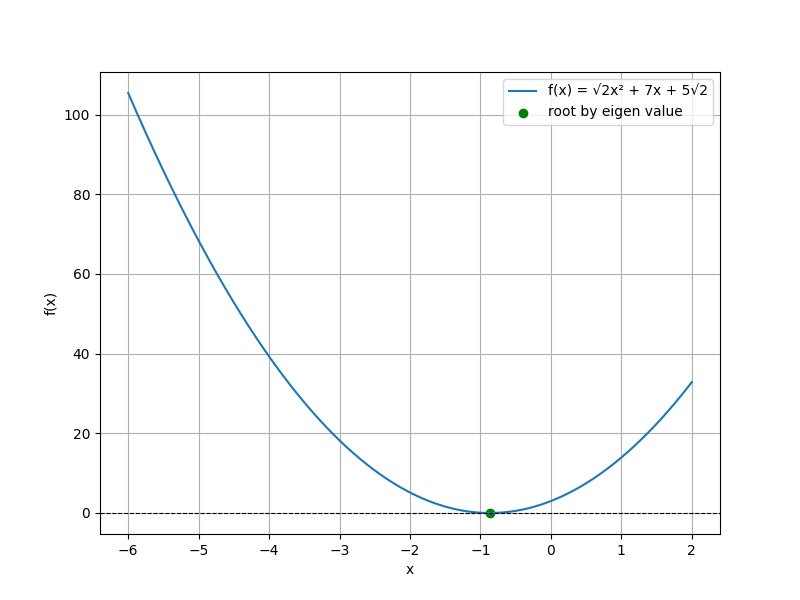
\includegraphics[width=0.7\linewidth]{figs/fig.png}
\end{figure}

\end{document}
